\documentclass[border=6pt,tikz]{standalone}
\usepackage{tikz}
\usepackage{amsmath,amssymb}
\usetikzlibrary{arrows.meta,positioning,fit,backgrounds,calc,shapes.geometric,decorations.pathreplacing,patterns}
\definecolor{ink}{HTML}{1B2430}
\definecolor{muted}{HTML}{6B7785}
\definecolor{accent}{HTML}{2F6FB5}
\definecolor{accent2}{HTML}{C1611F}
\definecolor{good}{HTML}{2E7D5B}
\definecolor{soft}{HTML}{EDF2F7}
\definecolor{soft2}{HTML}{FBEDE2}
\definecolor{soft3}{HTML}{E6F0E9}
\tikzset{
  box/.style={draw=ink,line width=.7pt,rounded corners=2pt,fill=soft,inner sep=4pt,align=center,font=\sffamily\small},
  boxa/.style={box,fill=soft2},
  boxb/.style={box,fill=soft3},
  plain/.style={align=center,font=\sffamily\small,text=ink},
  tiny/.style={align=center,font=\sffamily\scriptsize,text=muted},
  ar/.style={-{Stealth[length=2.4mm]},draw=ink,line width=.7pt},
  arm/.style={-{Stealth[length=2.4mm]},draw=muted,line width=.6pt,dashed},
  nd/.style={circle,draw=ink,line width=.7pt,fill=white,minimum size=7mm,inner sep=0pt,font=\sffamily\scriptsize},
  ndf/.style={nd,fill=soft},
  ndt/.style={nd,fill=soft2},
}

\begin{document}
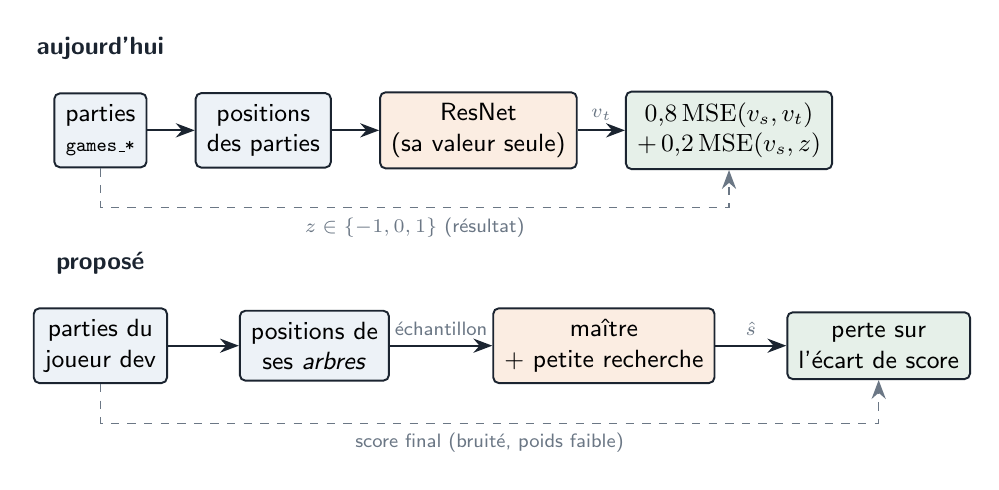
\begin{tikzpicture}[node distance=6mm]
  \node[plain,font=\sffamily\bfseries\small] (t1) {aujourd'hui};
  \node[box,below=3mm of t1] (g) {parties\\\scriptsize\texttt{games\_*}};
  \node[box,right=of g] (p) {positions\\des parties};
  \node[boxa,right=of p] (r) {ResNet\\(sa valeur seule)};
  \node[boxb,right=of r] (l) {$0{,}8\,\mathrm{MSE}(v_s,v_t)$\\$+\,0{,}2\,\mathrm{MSE}(v_s,z)$};
  \draw[ar] (g) -- (p); \draw[ar] (p) -- (r); \draw[ar] (r) -- node[tiny,above]{$v_t$} (l);
  \draw[arm] (g.south) -- ++(0,-5mm) -| node[tiny,below,pos=.25]{$z\in\{-1,0,1\}$ (résultat)} (l.south);

  \node[plain,font=\sffamily\bfseries\small,below=22mm of t1] (t2) {proposé};
  \node[box,below=3mm of t2] (g2) {parties du\\joueur dev};
  \node[box,right=9mm of g2] (p2) {positions de\\ses \emph{arbres}};
  \node[boxa,right=13mm of p2] (r2) {maître\\+ petite recherche};
  \node[boxb,right=9mm of r2] (l2) {perte sur\\l'écart de score};
  \draw[ar] (g2) -- (p2); \draw[ar] (p2) -- node[tiny,above]{échantillon} (r2); \draw[ar] (r2) -- node[tiny,above]{$\hat s$} (l2);
  \draw[arm] (g2.south) -- ++(0,-5mm) -| node[tiny,below,pos=.25]{score final (bruité, poids faible)} (l2.south);
\end{tikzpicture}
\end{document}
